\documentclass[a4paper, 12pt]{book}
% preamble.tex

\usepackage[utf8]{inputenc}
\usepackage[T1]{fontenc}
\usepackage[english]{babel} % Ho cambiato in italian, supponendo che la maggior parte del testo sia in italiano
\usepackage{amsmath}
\usepackage{amssymb}
\usepackage{graphicx}
\usepackage{hyperref}
\usepackage{geometry}
\usepackage{fontspec} % Utile per Xetex/LuaLaTeX ma mantenuto
\usepackage{booktabs}
\usepackage{amsthm}
\usepackage{enumitem}
\usepackage{caption}
\usepackage{thmtools}
\usepackage{standalone} % Già presente nel tuo elenco
\usepackage{tkz-euclide}
\usepackage{graphicx}
\usepackage[T1]{fontenc}
\usepackage{wesa}

% --- PACCHETTI AGGIUNTI PER LA FORMATTAZIONE ---
\usepackage{parskip}  % Aggiunge spazio tra i paragrafi (stile "blocco")
\usepackage{fancyhdr} % Per intestazioni e piè di pagina personalizzati

% --- IMPOSTAZIONI GEOMETRIA E FONT ---
\geometry{a4paper, margin=1in}

% Configura lo stile 'plain' (usato da \maketitle e \tableofcontents)
% per essere coerente con il piè di pagina
\fancypagestyle{plain}{
    \fancyhf{} % Pulisce
    \cfoot{\thepage} % Mette solo il numero di pagina
    \renewcommand{\headrulewidth}{0pt} % Niente linea su queste pagine
}

% Configurazione Header/Footer per le altre pagine
\pagestyle{fancy}
\fancyhead{} % Pulisce l'intestazione
\fancyfoot{} % Pulisce il piè di pagina
\fancyhead[L]{\nouppercase{\rightmark}} % Nome Sezione a sinistra (o Chapter)
\fancyhead[R]{\nouppercase{\leftmark}}  % Nome Capitolo a destra (o Sezione)
\fancyfoot[C]{\thepage} % Numero di pagina al centro
\renewcommand{\headrulewidth}{0.4pt}
\renewcommand{\footrulewidth}{0pt}


% --- DEFINIZIONI TEOREMI ---
% (Questa parte è cruciale per la tua struttura)
\newtheoremstyle{mythmstyle}%
    {}%
    {}%
    {\itshape}%
    {}%
    {\bfseries}%
    {}%
    { }%
    {\thmname{#1}\thmnumber{ #2}%
    \thmnote{: #3\addcontentsline{toc}{subsubsection}{{\itshape#1}: #3}}. }

% 2. Imposta questo stile come quello ATTUALE
\theoremstyle{mythmstyle}

\newtheorem{theorem}{Th}[section]
\newtheorem{definition}{Def}[section]
\newtheorem{proposition}{Prop}[section]
\newtheorem{corollary}{Cor}[section]
\newtheorem{algorithm}{Alg}[section]
\newtheorem{lemma}{Lemma}[section]
\newtheorem*{remark}{Rem}

% Definizioni utili per il Main file
\newcommand{\inputlesson}[1]{\clearpage\input{#1}\clearpage} % Comando per input lezione

\usepackage{tikz}
\usetikzlibrary{shapes,fit}
\usepackage{amsmath} % Required for align environment
\usepackage{caption} % Required for \captionof outside float environments



\begin{document}
\setcounter{chapter}{9}
\chapter{Lesson 5-12-2025}
% Stile per la barra verde verticale a sinistra (Note/Definizioni)


% --- INIZIO DEL CONTENUTO ---
\section{Channel modeling}

\subsection[Friis' equation]{Friis' equation and discussion on the choice of the transmission frequency}

Let's say we have

\begin{figure}[h]
    \centering
    % [IMAGE PLACEHOLDER: Diagram of Transmitter, Scatterer, Diffraction, Reflection, Receiver 0/1]
    
\includegraphics[width=0.5\textwidth]{Pictures/image.png}
\end{figure}

Which parameters do we need?
The gains of the transmit and receive antennas: $G_T, G_R$.

\begin{bluebox}[\faPen\ Friis' equation]
What's the equation which binds the two?
\begin{align*}
P_r = P_t G_t G_r \frac{1}{d^2 f^2} \left(\frac{c}{4\pi}\right)^2 = P_t G_t G_r \left(\frac{\lambda}{4\pi d}\right)^2 \,;
\end{align*}
this is Friis' equation; what does this tell us?
\end{bluebox}

We can't do anything on the distance! \textbf{We can do something on the frequency} though; if we double the frequency, the received power will be divided by 4.
The lower frequencies will be the best ones. Of course we can't go baseband: the size of the antenna is somehow proportional to $\lambda$; if we have $f=0$, we'll need to have $\lambda = \infty$ and thus we'd need an extremely large antenna.

In Europe the unlicensed band is around \textbf{868MHz}. We then have other ones at \textbf{2.4, 5GHz}: those are used by the wifi.
If we have a router and home, let's imagine we have a switch between the two; normally it transmits at both. When we transmit, we can decide which to use; we might think we'll certainly choose 2.4GHz, since it will get 4 times the power the other gives!
There are other considerations; speed is something we want: the bitrate does not only depend on the power, but also on the bandwidth. Here the bandwidth is larger. At 5GHz we have \textbf{higher bitrate but more attenuation}, while at 2.4GHz we don't have as much attenuation but we also have a lower bandwidth.

If we consider the channel itself, it would prefer lower frequencies. It's also true that \textbf{sometimes we want attenuation} (voice is attenuated: we can talk without disturbing the neighbour by lowering the voice).

\begin{greenbar}
We don't want the router of our neighbour to enter our house, as that would create interference. The fact that the waves are attenuating is good, if we look at that kind of principle.
\end{greenbar}

Here the exponent is 2.
We know that now wifi is converging towards mmwaves; these are frequencies for which the $\lambda$ is comparable with \textbf{1mm}, meaning that the frequency is $f > \textbf{6GHz}$.
Why so? mmwaves have some other problems; if we are in the air (not in the free space anymore), we have oxygen, water, \dots
If we take a frequency which is resonating certain molecules, then we have peaks of absorption at certain frequencies. The frequencies at mmwaves experience the phenomenon of \textbf{blockage}. If the wave just meets a leaf, it's immediately blocked. Such high frequencies (like mmwaves) are blocked by many types of obstacles.
Point is that higher frequencies have very large and non-crowded bandwidth: if we're in line of sight, we can upload gigabits per second!

Of course the more bandwidth we have, the larger the bitrate we can achieve (this follows easily from $R/B = C$: for a fixed capacity, increasing the bandwidth gives us a better bitrate).
Let's suppose we can get the line of sight.

If we consider that each cellular phone has a bandwidth of 2MHz, this means that
\begin{align*}
\frac{60\text{GHz}}{2\text{MHz}} = 3 \cdot 10^4
\end{align*}
(where $60\text{GHz}$ is the frequency of one of the more recent standards) this is a really big attenuation factors; how can we do this, then? 5G is using mmwaves; 6G is thinking of THz! We solve the problem of the high attenuation by working on the gain of antennas; amplifiers are not the way, as they introduce noise; the antennas are passive elements.

\begin{figure}[h]
    \centering
    % [IMAGE PLACEHOLDER: Diagram of Transmitter, Scatterer, Diffraction, Reflection, Receiver 0/1]
    
\includegraphics[width=0.5\textwidth]{Pictures/image copy.png}
\end{figure}

Since we have mmwaves, we can make an antenna which is just of the size of a millimiter; we can thus have multiple small antennas in a very small area.
Going back again: we can set the gains really high. This is like directing the power specifically in a certain direction.

\begin{greenbar}
The gain comes from the fact that the signal is propagating specifically in one direction.
\end{greenbar}

\begin{greybox}[\faQuoteLeft\ In-class stuff]
THz is really horrible; generally telecommunications have always been like: "we make this, somebody will use it"; now telecommunications has a market pull: they say \textit{we need something} and we're the ones finding such things.
The use case for THz waves is to replace the cables in data centers. This would allow for great simplifications in situations with many cables.

\begin{greenbar}
Shows a picture with attenuation depending on the transmission frequency.
The spots of minima are candidates for 5G; wifi instead uses the spots where attenuation is higher; this is because wifi knows it does not need to go far in distance.
The maximas are used depending on the application; if we just need low distance transmission, we can use the maxima as well.
\end{greenbar}

Now we should have an idea of how the frequencies are selected. There is a lot of discussion about the human damages which according to certain people are being cause by electromagnetic waves.

\begin{greenbar}
Controversy of people not wanting 5G; we have a parameter called SAR (specific absorption rate): we can't commercialize stuff which has wrong values of this.
In principle, high frequencies on molecules should not be more dangerous than the lower ones; actually, the low frequencies are even worse.
\end{greenbar}
\end{greybox}

\section{Modeling approaches}

\subsection{Modeling of radio propagation (LOS, NLOS, effects on the signals)}

\textit{Handwritten note: Two approaches $\to$ deterministic $\to$ ray tracing (difficult) (GPU). Stochastic $\to$ lights... used for underwater communications.}

Highlights; we'll skip them.

Propagation modeling; there are different effects that we should take into account. The aim is to develop a mathematical model of what happens physically!

The best that can happen is that our signal directly reaches the receiver, through a line of sight (LOS); generally, what happens is that the signal actually reaches the receiver through some different type of path, aka a non-line of sigh (NLOS).
We have different possibilities, when it comes to NLOS:

\begin{enumerate}
    \item A wave might bounce off a smooth object of size exceedingly large relative to the wavelength of the signal: we have \textbf{reflection}; each incoming wave is mapped onto a single reflected direction.
    \item \textbf{Scattering} is said to have occurred when a wave travels through a medium that contains objects whose dimensions are smaller than or comparable to the wavelength, and where the number of such objects is large. Then, each incoming wave is mapped onto many scattered ones.
    \item Radio waves also bend around sharp edges, a phenomenon that is referred to as \textbf{diffraction} and that plays a pivotal role in urban settings. Indeed, a major contributor to the propagation of radio signals in such settings is rooftop diffraction.
\end{enumerate}

\begin{figure}[h]
    \centering
    % [IMAGE PLACEHOLDER: Diagram of Transmitter, Scatterer, Diffraction, Reflection, Receiver 0/1]
    
\includegraphics[width=0.8\textwidth]{Pictures/immagine-000.png}
    \caption*{Ray tracing example: Reflection, Scattering, Diffraction}
\end{figure}

The Maxwell equations are not enough to describe the various effects we can have, such as diffraction, reflection, scattering. Only if we're lucky do we have a line of sight.
In order to solve this we'd need to solve differential equations which are exceedingly more complicated: we could not get out of that, not even with super computers.

\begin{bluebox}[\faPen\ Clutter]
In an urban scenario, we refer to the \textbf{propagation clutter} as the set of objects which cause the NLOS effects; we can have either an elevated transceiver (if it's elevated with respect to the clutter) or a \textit{within clutter} transceiver.
\end{bluebox}

We'll then derive an abstraction simple enough for us to be able to handle the model, but also complicated enough to be able to capture the major effects which are happening.
Such a model is key of information engineering.
We always need to be careful about the conditions which allowed us to form the model.

% --- FINE PAGINA 04 / INIZIO PAGINA 05 ---
\newpage

It's difficult (impossible!) that things go better than what is predicted by the Friis equations, which only work in line of sight.
We'll then develop a mathematical description of multi-path propagation channels inspired by propagation channel measurements.

\begin{bluebox}[\faPen\ Sensitivity of the receiver]
\textbf{Sensitivity of the receiver}: the minimum amount of power needed to correctly receive a signal with a certain probability.
Sensitivity of -100dBm; if we receive any greater power, we'll receive the signal and interpret it correctly with a good probability.
We have very expensive softwares able to map a whole area this way.
It's also true that "high power signal" does not mean that we have a clean signal.
\end{bluebox}

\subsection{Modeling approaches (deterministic, stochastic); elements of the modelization}

We know that in the end we won't generally develop a deterministic model, as that would be extremely complicated (involving ray tracing and such); we only do this sometimes, like with millimeter waves (since they generally require ray tracing of indoor sites). More often, we do stochastic models!

\begin{figure}[h]
    \centering
    % [IMAGE PLACEHOLDER: Comparison between Deterministic (Ray tracing) and Stochastic (Received power graph) models]
    
\includegraphics[width=0.8\textwidth]{Pictures/immagine-001.png}
    \caption*{Deterministic vs Stochastic approaches}
\end{figure}

\begin{yellowbox}
\faBook\ \textit{Channel modeling (pp. 131-208), page 4}

In general, a stochastic model is embodied by the \textbf{conditional distribution of the channel output given its input}. When the channel is linear, as is the case in the wireless medium, this is tantamount (\textit{equivalente}) to a stochastic impulse response.
\end{yellowbox}

A critical distinction which needs to be made when modeling is that between large-scale and small-scale phenomena.

\begin{yellowbox}
\faBook\ \textit{Channel modeling (pp. 131-208), page 4}

Specifically, what is \textbf{assumed is that the distribution of the channel response is locally stationary within certain neighborhoods around transmitter and receiver}.
\end{yellowbox}

We'll just assume wide-sense stationarity, but we might as well assume strict-sense stationarity.
The neighborhoods in which the signal can be considered to be stationary is generally in the order of tens to hundreds of wavelengths.

% --- FINE PAGINA 05 / INIZIO PAGINA 06 ---
\newpage

\begin{yellowbox}
\faBook\ \textit{Channel modeling (pp. 131-208), page 4}

\textbf{Large-scale phenomena impact} the local distribution to which the small-scale phenomena conform, \textbf{generally the local-average power}.
\end{yellowbox}

\begin{yellowbox}
\faBook\ \textit{Channel modeling (pp. 131-208), page 5}

Because of the importance of the decoupling of large- and small-scale phenomena, we use distinct variables to model them and carry those throughout the derivations in the entire book. While this takes a small toll in terms of the compactness of some expressions, it reinforces the separation between quantities that change at very different scales in time and frequency, and which have markedly different effects on the communication.
\end{yellowbox}

Just an insight on the approach we'll further discuss later: we generally draw a regression line trying to minimize the distance between the line and the various values.
We make great campaigns of measurements, in order to obtain sufficient data to model this. We then decompose everything in two (+1) components:

\begin{enumerate}
    \item \textbf{Large-scale fading}: if we go around the corner, we have another propagation, changing abruptly; this depends heavily on where we are! This change is not smooth.
    \item \textbf{Small-scale fading}: depends on how the various waves come to the receiver and how they arrive at the receiver; if we move our phone up and down, we'll have variations in the signal.
    \item \textbf{Line loss}: this changes depending on what we have in-between. There are parameters to tune if the loss is due to walls, ceilings, iron, \dots; this needs to be managed carefully.
\end{enumerate}

\begin{figure}[h]
    \centering
    % [IMAGE PLACEHOLDER: Graph showing Pathloss, Shadow fading, Small-scale fading vs Distance]
    
\includegraphics[width=0.8\textwidth]{Pictures/immagine-002.png}
    \caption*{Decoupling of fading types over distance}
\end{figure}

In MIMO, we want to have full-rank matrices; small scale fading can help to make the various matrices full rank!

\section{Large scale phenomena}
% --- INIZIO PAGINA 07 ---

\subsection{Pathloss and shadow fading (their separation, distribution of the shadow fading), pathloss; large-scale channel gain $G$ and partial values $P_t, P_r, G_t, G_r$}

\begin{yellowbox}
\faBook\ \textit{Channel modeling (pp. 131-208), page 5}

Under the separation argued in the previous paragraph, large-scale phenomena are those that determine the local distribution of the stochastic channel response. The prime feature of that distribution is, of course, the power. If one plots, for a given transmit power, the local-average received power (in log-scale) obtained from many empirical measurements in otherwise identical conditions as a function of the distance (also in log-scale) between transmitter and receiver, the result is invariably a cloud of scattered points, such as the one in the figure below

\begin{center}
    % [IMAGE PLACEHOLDER: Scatter plot showing Pr(dB) vs log D with a regression line]
    
\includegraphics[width=0.6\textwidth]{Pictures/immagine-004.png}
\end{center}
\end{yellowbox}

The line we see in the figure above is a linear regression line which relates the local-average received power to the distance. Such a law represents what we call the \textbf{pathloss}, which we'll denote as $L_p$; the scattered measurements around the law is what we call \textbf{shadow fading}, denoted by $\chi$.
The pathloss and the shadow fading put together give the large-scale description of virtually every existing channel model.

\begin{yellowbox}
\faBook\ \textit{Channel modeling (pp. 131-208), page 6}

Although recent work indicates, on solid analytical footings based on random walks and diffusion theory, that nonlinear regressions may sometimes be superior [203, 204], the \textbf{combination of pathloss and shadow fading suffices for our purposes}.
\end{yellowbox}

\begin{yellowbox}
\faBook\ \textit{Channel modeling (pp. 131-208), page 6}

The pathloss can be interpreted as the expected attenuation over an ensemble of realizations of a given propagation scenario, whereas the shadow fading individualizes, through randomization, the attenuation of each such potential realization.
\end{yellowbox}

% --- FINE PAGINA 07 / INIZIO PAGINA 08 ---
\newpage

\begin{yellowbox}
Another common interpretation of the large-scale phenomena is that the \textbf{pathloss quantifies the local-average attenuation} tied exclusively to distance whereas the \textbf{shadow fading accounts for the presence of obstacles} that cause the local-average attenuation to deviate from the value predicted by the pathloss. This is illustrated in Fig. 3.4 (below here), which depicts how both pathloss and shadow fading affect the evolution of the received signal power as the distance between transmitter and receiver increases over a generic trajectory; the pathloss is monotonic, whereas the shadow fading can oscillate as obstacles come in and out of the way. It was suggested in [205] that \textbf{the shadow fading attenuation, $\chi$, could follow a lognormal distribution} and empirical measurements have repeatedly confirmed the excellent fit to data offered by such distribution [206, 207]. The most widely accepted justification for this log-normal nature is that shadow fading represents the product of the losses introduced by the several obstacles traversed by the signal and, in log-scale, such a product becomes a sum of independent terms. Despite the fact that those terms can hardly be assumed to conform to the same distribution, and that the number of such terms may not be particularly large, the robustness of the central limit theorem (see Appendix C.1.10) renders the sum surprisingly well modeled by a Gaussian random variable.

\begin{center}
    % [IMAGE PLACEHOLDER: Fig 3.4 Graph showing Pathloss (smooth curve), Shadow fading (jagged curve), and Small-scale fading (high freq noise)]
    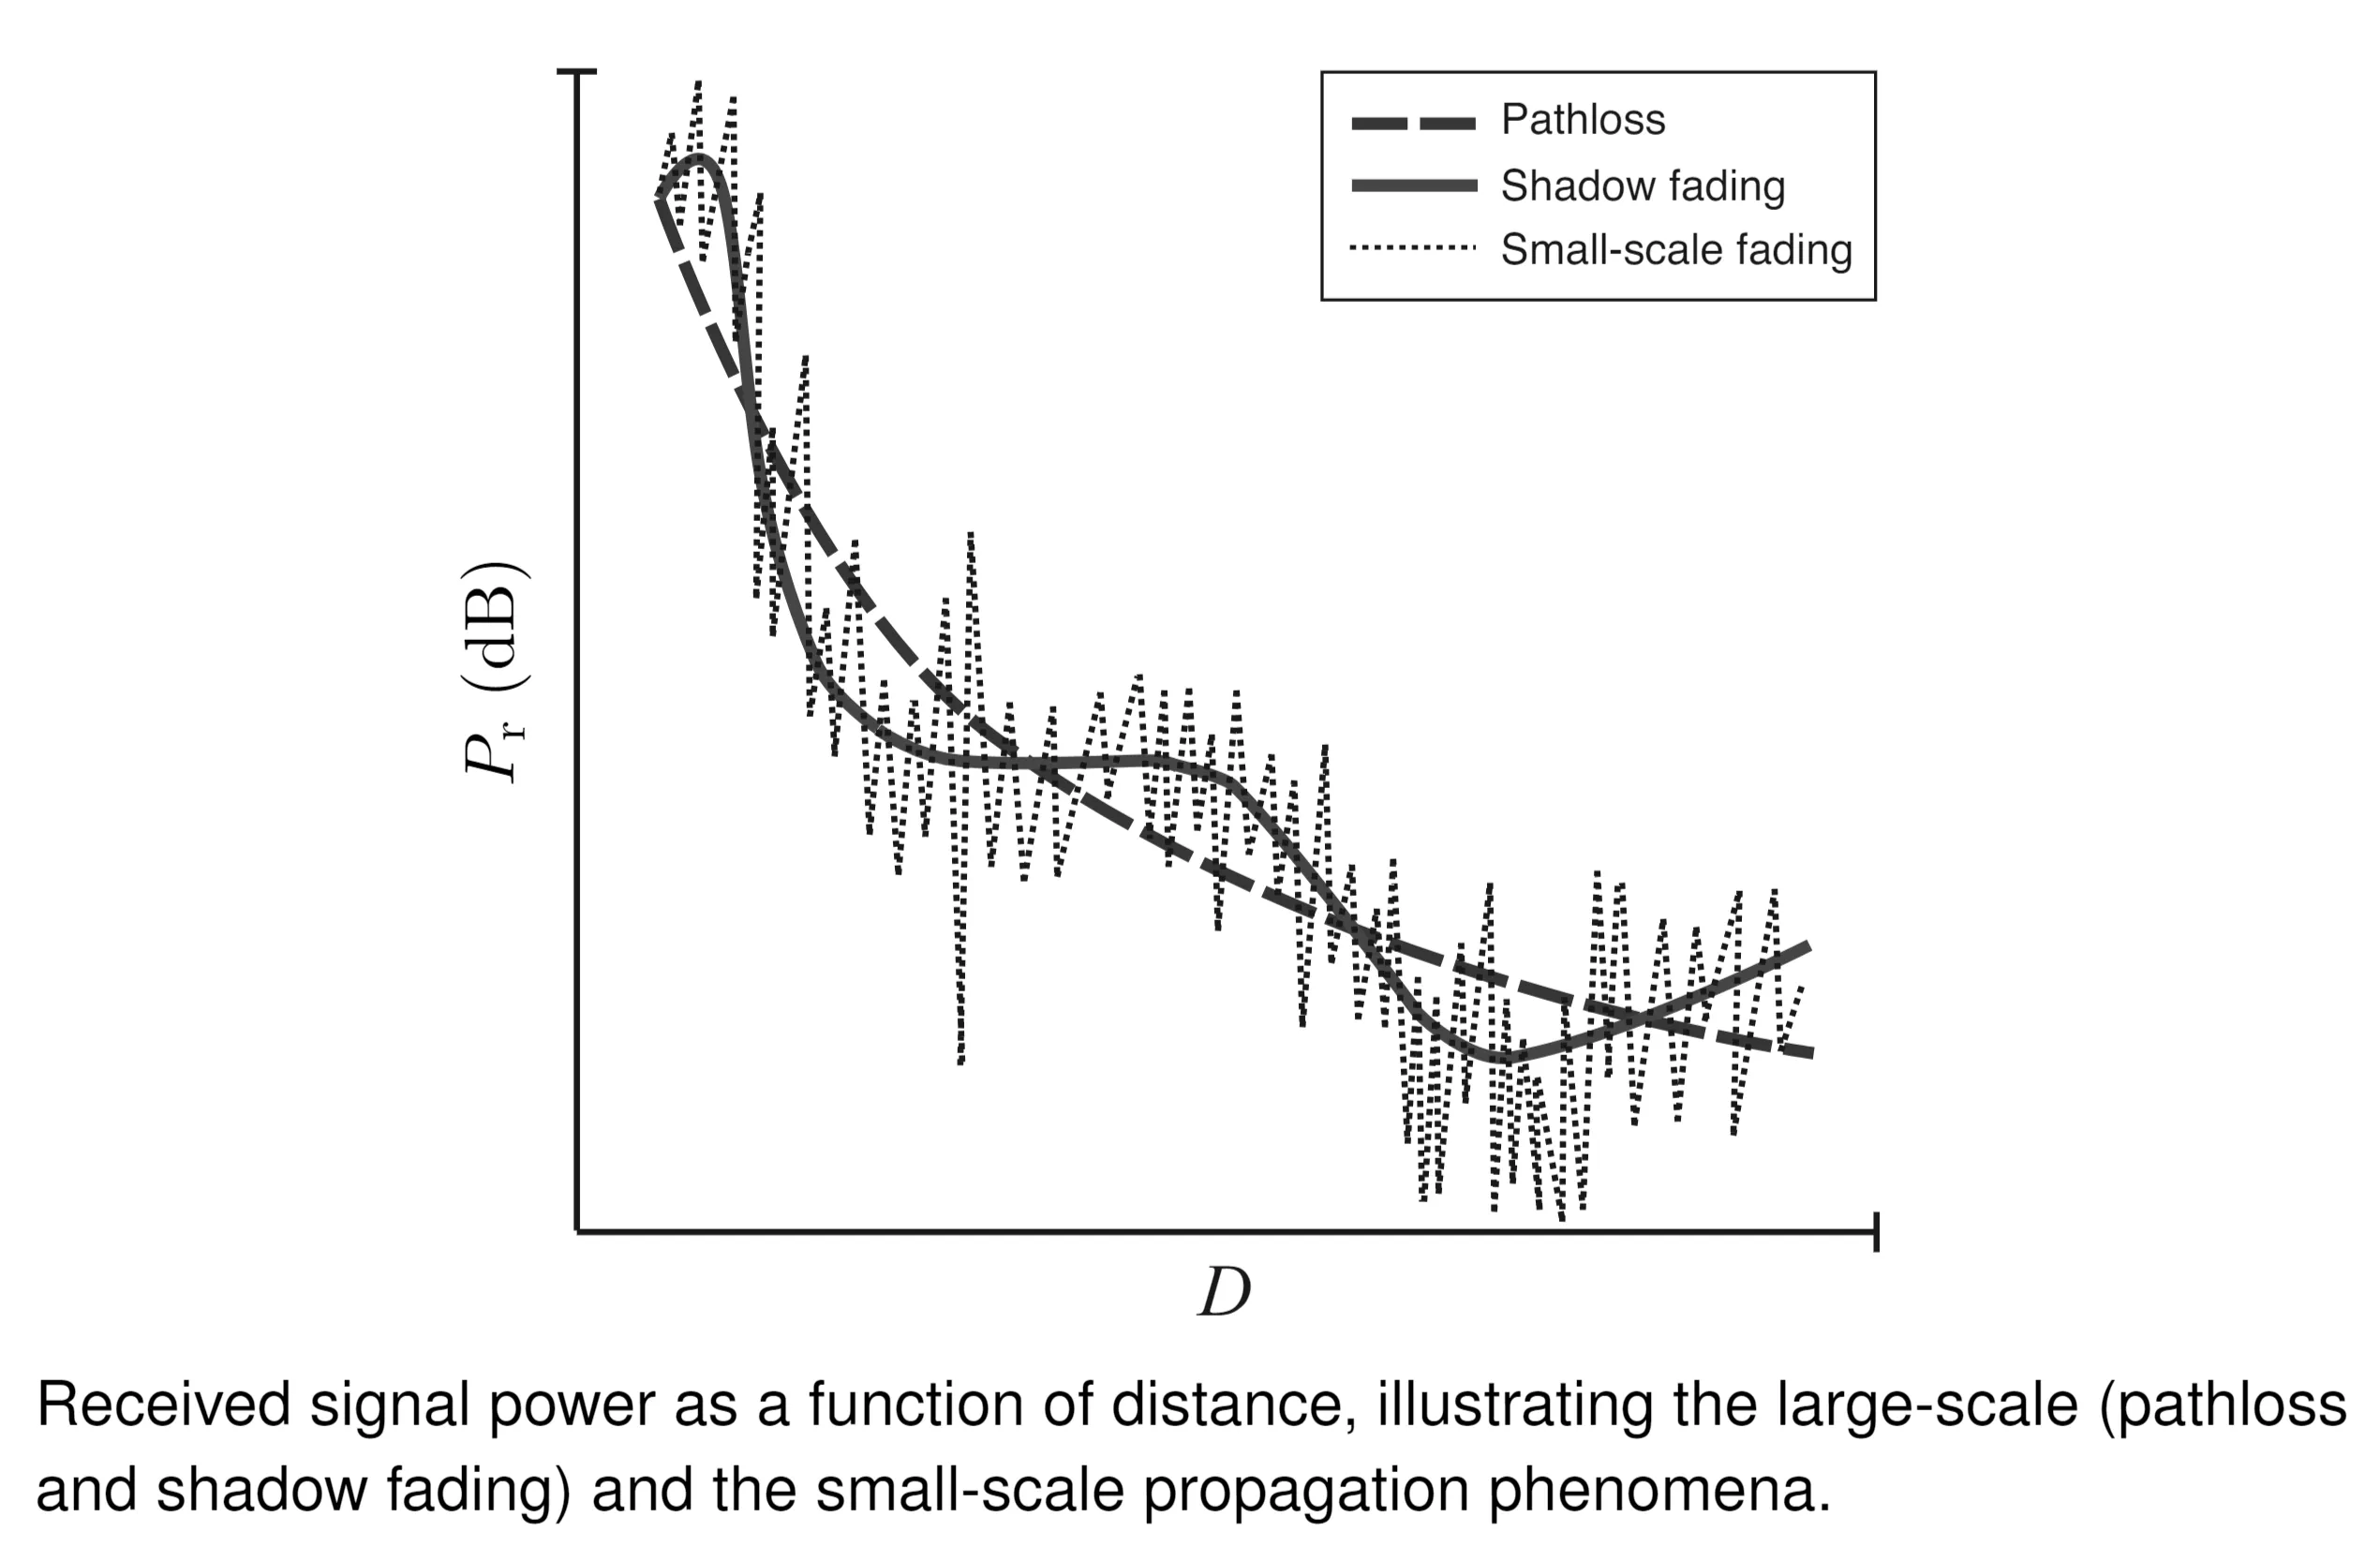
\includegraphics[width=0.6\textwidth]{Pictures/immagine-005.png}
    \captionof{figure}{Received signal power as a function of distance, illustrating the large-scale (pathloss and shadow fading) and the small-scale propagation phenomena. Fig. 3.4}
\end{center}
\end{yellowbox}

We thus have that under the log-normal model, $\chi|_{\text{dB}}$ is Gaussian with PDF
\begin{align}
f_{\chi|_{\text{dB}}}(\xi) = \frac{1}{\sqrt{2\pi}\sigma_{\text{dB}}} \exp \left( - \frac{\xi^2}{2\sigma_{\text{dB}}^2} \right) \,, \tag{3.1}
\end{align}
where $\sigma_{\text{dB}}$ is the standard deviation which is generally assumed to be independent of the distance for the sake of simplicity.

\begin{yellowbox}
\faBook\ \textit{Channel modeling (pp. 131-208), page 7}

Outdoors, $\sigma_{\text{dB}}$ tends to range between 8 and 12 dB. Indoors, it is usually smaller.
\end{yellowbox}

\begin{greenbar}
Log-normal random variable is like a Gaussian in the log domain! We use a Gaussian because it is given by the summing of various different random variables.
\end{greenbar}

% --- FINE PAGINA 08 / INIZIO PAGINA 09 ---
\newpage

The signal was represented as zero-mean: we can easily include a mean in the log-scale Pathloss.
We can also rewrite the distribution in linear scale, see \textcolor{green!60!black}{08.3\_pp\_131\_208\_Channel\_modeling, page 7}.

\begin{yellowbox}
\faBook\ \textit{Channel modeling (pp. 131-208), page 7}

A relevant property confirmed through empirical observations is that, as intuition would have it, shadow fading \textbf{can be broken up into distinct pieces: one} that depends on the \textbf{location of the transmitter} and \textbf{one} that depends on the \textbf{location of the receiver} [207]. Two mutually distant receivers communicating with the same transmitter (or two mutually distant transmitters communicating with the same receiver) experience the same shadow fading for one piece but a completely different shadow fading for the other. These two pieces, whose values add up in log-scale, tend to have similar strengths. Furthermore, measurements reported in [208] point to an exponential model for the spatial autocorrelation of each piece, with a correlation distance that is on the order of tens of meters outdoors, depending on the environment, and substantially shorter indoors [209]. For more refinements on the modeling of shadow fading, the reader is referred to [210, 211] and references therein.
\end{yellowbox}

We can express the local-average received power $P_r$ as a balance of gains and losses according to the \colorbox{yellow!30}{link budget equation}:

\begin{equation}
\colorbox{yellow!10}{$\displaystyle P_r|_{\text{dB}} = P_t|_{\text{dB}} + G_t|_{\text{dB}} + G_r|_{\text{dB}} - (\underbrace{L_p|_{\text{dB}} + \chi|_{\text{dB}}}_{\text{Pathloss function}}) \,,$} \quad \xrightarrow{\text{better to measure it in dBm}} \tag{3.4}
\end{equation}

It's somewhat like the Friis equation; we have the plus operation because we're in the log domain.

\begin{minipage}{0.65\textwidth}
We can also rewrite it \colorbox{yellow!30}{more compactly as}
\begin{align}
P_r|_{\text{dB}} = P_t|_{\text{dB}} + G|_{\text{dB}} \,, \tag{3.5}
\end{align}
where \colorbox{yellow!30}{the gain}
\begin{align}
G = \frac{G_t G_r}{L_p \chi} \tag{3.6}
\end{align}
\end{minipage}
\hfill
\begin{minipage}{0.3\textwidth}
    \footnotesize
    \textbf{Why they created logs?} \\
    In math, to "convert" products to sums.
    \[ \log(a \cdot b) = \log(a) + \log(b) \]
    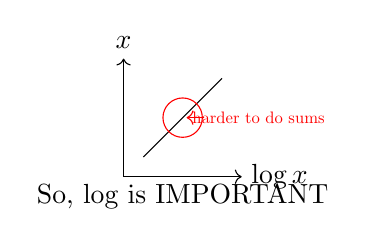
\begin{tikzpicture}[scale=0.5, baseline]
        \draw[->] (0,0) -- (0,3) node[above] {$x$};
        \draw[->] (0,0) -- (3,0) node[right] {$\log x$};
        \draw (0.5, 0.5) -- (2.5, 2.5);
        \node at (1.5, -0.5) {So, log is IMPORTANT};
        \node[draw, circle, red, minimum size=0.5cm] at (1.5, 1.5) {};
        \draw[red, ->] (2, 1.5) -- (1.6, 1.5) node[right, red, scale=0.6] {harder to do sums};
    \end{tikzpicture}
\end{minipage}

\vspace{1em}
is the \textbf{large-scale channel gain}, a quantity which was already introduces in the signal processing section to normalize the channel response; only now it is acquiring its full significance.
Of course if we have a log, the exponent can change.

\section{Two-exponents model}

\colorbox{yellow!30}{We then have} another \colorbox{yellow!30}{path loss modeling}; it gives the loss depending on the distance, which only applies after a certain reference distance $D_{ref}$. We have an exponent $\eta$, which is normally higher than 2 and is called the pathloss exponent. We can also write this in dB:
% --- INIZIO PAGINA 10 ---
\begin{align}
L_p(D) &= K_{\text{ref}} \left( \frac{D}{D_{\text{ref}}} \right)^\eta \tag{3.7} \\
L_p(D)|_{\text{dB}} &= K_{\text{ref}}|_{\text{dB}} + 10\eta \log_{10} \left( \frac{D}{D_{\text{ref}}} \right) \quad D > D_{\text{ref}} \tag{3.8}
\end{align}
with $D_{\text{ref}}$ being the reference distance and $K_{\text{ref}}$ being the pathloss at $D_{\text{ref}}$.

\begin{greenbar}
This is a very rudimental model; we're only looking at the path loss.
\end{greenbar}

\begin{greenbox}[\faBookmark\ Values of $K_{\text{ref}}$]
If no value is specified for $K_{\text{ref}}$, it's safe to assume we can use the freespace value, as described in (3.9).
\end{greenbox}

\begin{yellowbox}
\faBook\ \textit{Channel modeling (pp. 131-208), page 8}

The exponent $\eta$ is the most consequential parameter, with typical values ranging between 3.5 and 4 if either the transmitter or the receiver are elevated. If both are within the propagation clutter, higher values can be encountered. Values below 2 are rare but possible in settings such as indoor corridors, outdoor urban canyons, or tunnels.
\end{yellowbox}

\begin{yellowbox}
\faBook\ \textit{Channel modeling (pp. 131-208), page 8}

The parameter $K_{\text{ref}}$ is sometimes referred to as the intercept at $D_{\text{ref}}$ because it is the value at which a plot of $L_p(D)$ intercepts a vertical axis drawn at $D_{\text{ref}}$. Given a reference distance, $K_{\text{ref}}$ can be measured empirically. Alternatively, if the reference distance is chosen properly, $K_{\text{ref}}$ can be computed under the assumption that the propagation from the antenna up to that point follows the free-space law described next. In this case, the representation in (3.8) becomes the two-slope model in Fig. 3.5 (\textit{see below here}), namely \textbf{free-space decay} up to $D_{\text{ref}}$ and decay \textbf{with exponent $\eta$ thereafter}. This two-slope behavior can be justified analytically [51, section 2.4.1] and on the basis of experimental observations [213]. Besides the representation in (3.8), suitably complemented by log-normal shadow fading, several pathloss modeling alternatives are available. These alternatives are the subject of the remainder of this section. While the focus here is exclusively on how the large-scale propagation phenomena affect the local-average received power, models do exist for how other features of the local distribution (introduced later in this chapter) are affected, e.g., the Rice factor, the power delay profile, or the angle spread [214, 215].
\end{yellowbox}

% --- FINE PAGINA 10 / INIZIO PAGINA 11 ---
\newpage

\begin{figure}[h]
    \centering
    % [IMAGE PLACEHOLDER: Fig 3.5 - Graph of Pr(dB) vs log D showing two slopes: Exponent 2 (free space) then Exponent eta]
    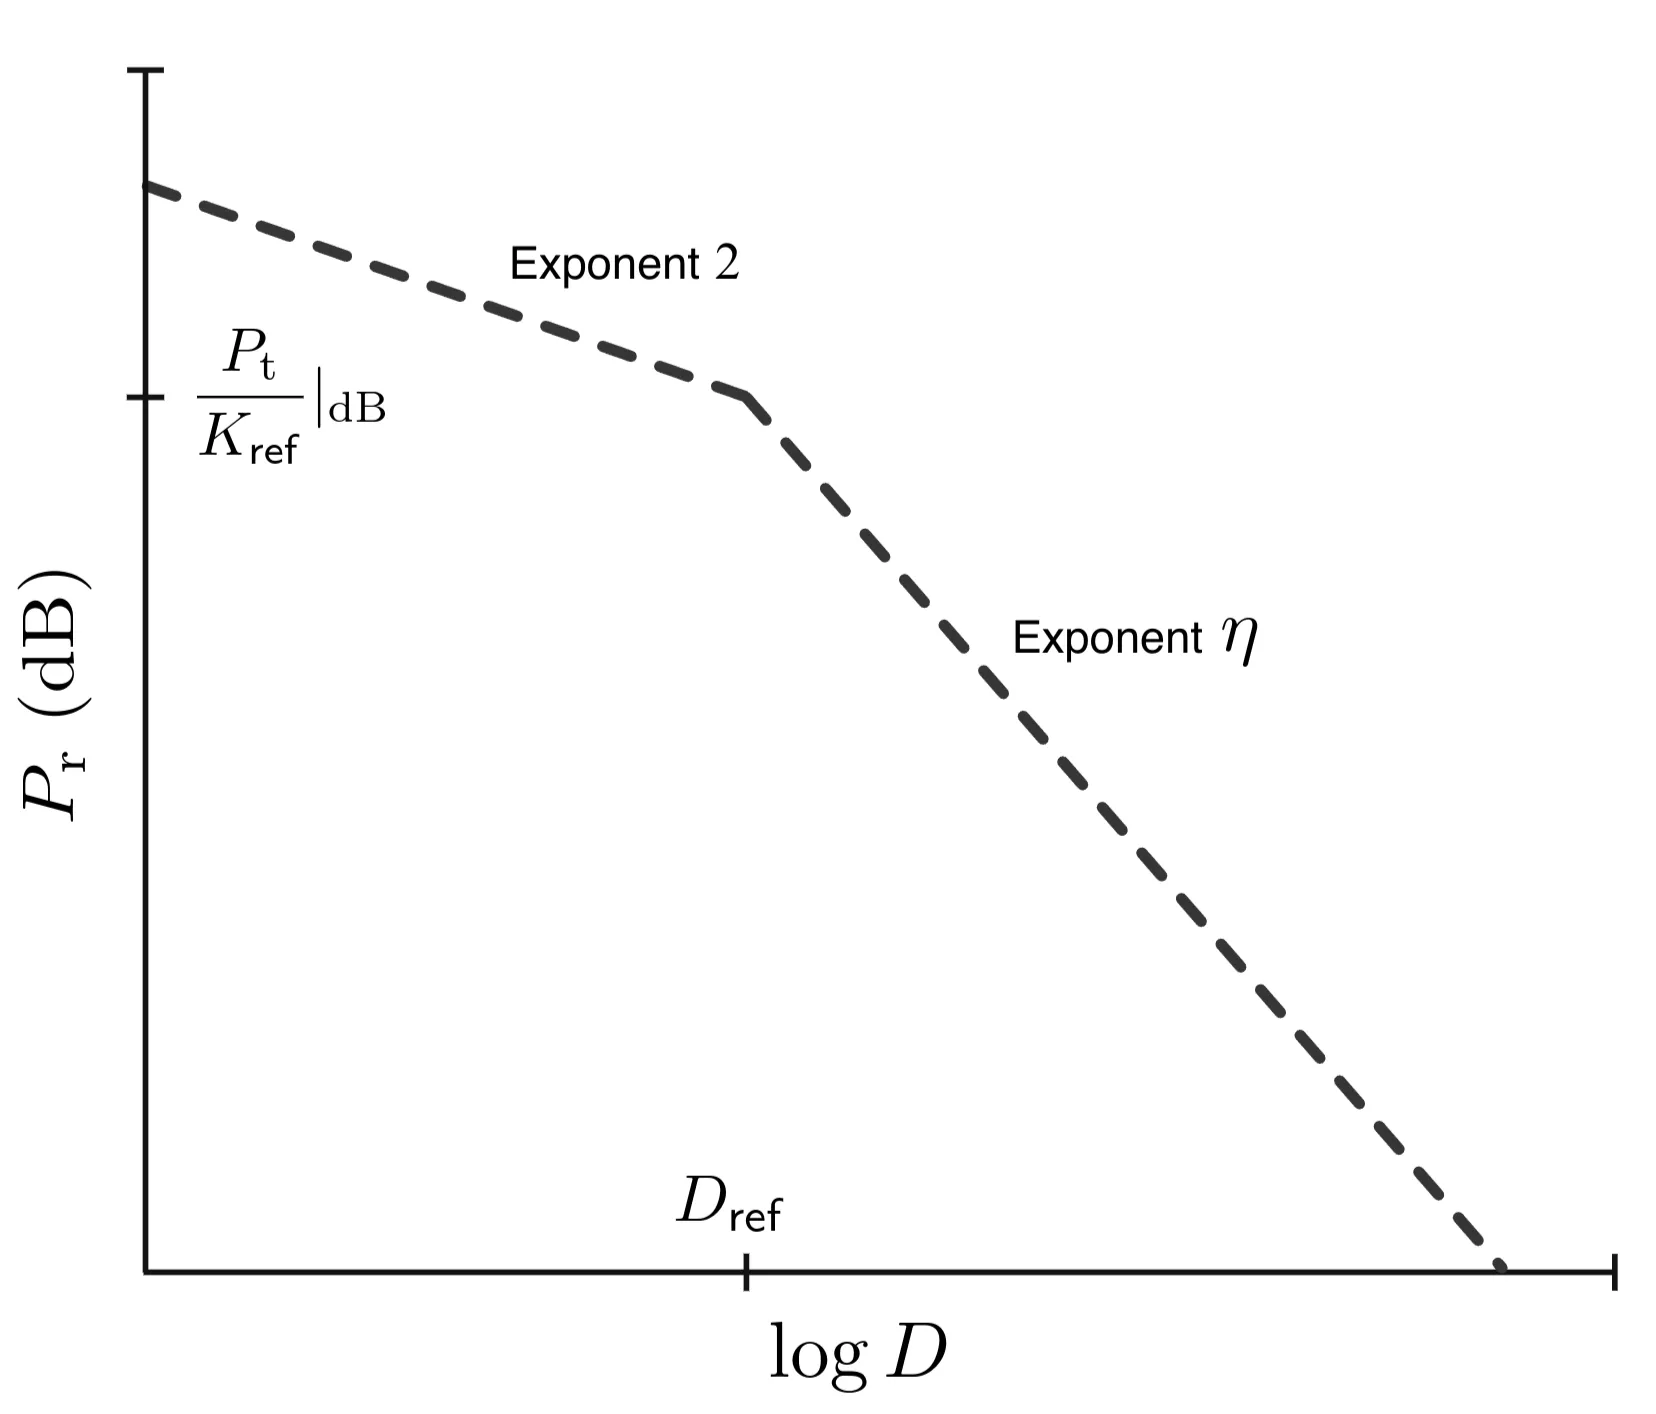
\includegraphics[width=0.7\textwidth]{Pictures/immagine-006.png}
    \caption*{Fig 3.5}
\end{figure}

The first slope in the figure 3.5 is the \textbf{pathloss in free space}, given by

\begin{align}
L_p(D)|_{\text{dB}} = 20 \log_{10} \left( \frac{4\pi D}{\lambda_c} \right) \,, \tag{3.9}
\end{align}

which is none other than (3.8) adapted with $K_{\text{ref}} = 1$ and $\eta = 2$; $\lambda_c$ is the carrier wavelength.

It \textbf{holds only when $D$ lies in the far-field region of the antennas}, the rule of thumb being $D \ge 2d_a^2/\lambda_c$ where $d_a$ is the largest physical dimension of either antenna. By definition, this model applies \textbf{only when there are no obstructions between transmitter and receiver or in the vicinity} of the trajectory linking them; this restricts its applicability to very specific situations, e.g., the computation of the intercept at a nearby point. There is no accompanying shadow fading. The presence of objects of any kind, even simply the ground, alters the square-law distance decay in (3.9), yielding a more general exponent $\eta$.

\begin{bluebox}[\faPen\ In class]
We also have a two-slope model: up to a certain distance we have an exponent; then we have another exponent $\eta$:
\end{bluebox}

% --- FINE PAGINA 11 / INIZIO PAGINA 12 ---
\newpage

\begin{figure}[h]
    \centering
    % [IMAGE PLACEHOLDER: Detailed diagram of Two-slope model with annotations (Free space assumed up until Dref...)]
    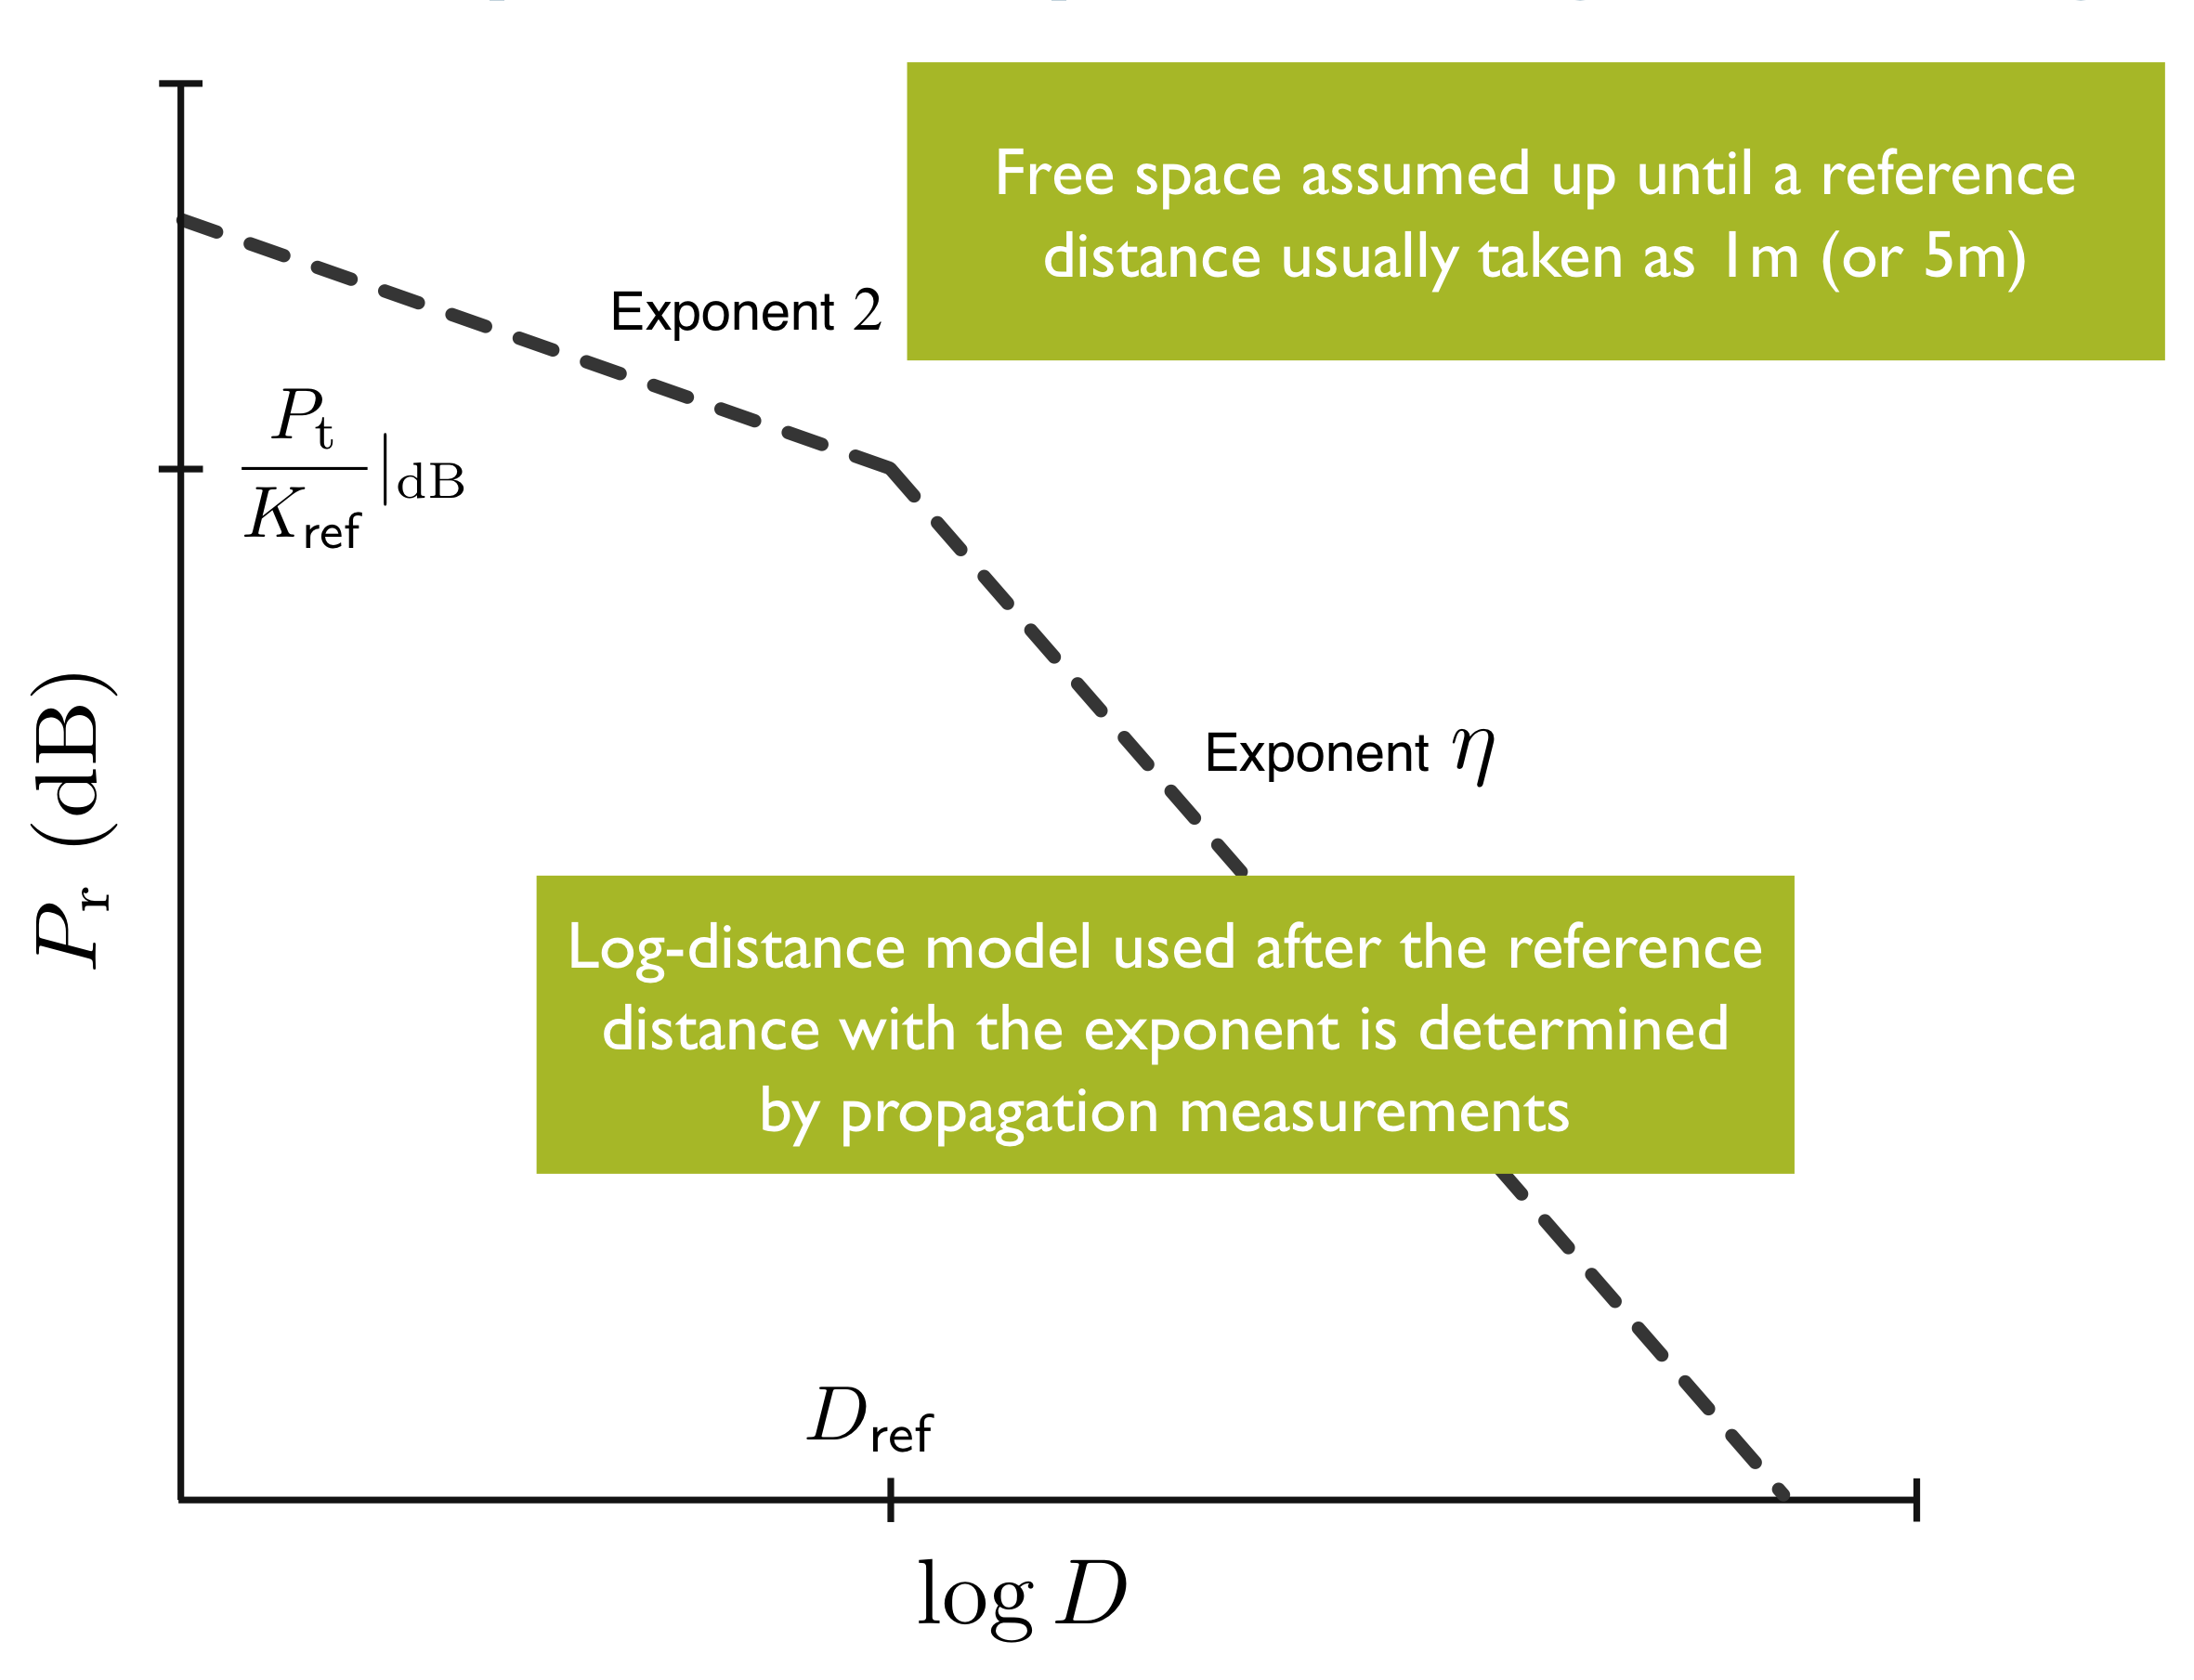
\includegraphics[width=0.8\textwidth]{Pictures/immagine-007.png}
\end{figure}

If we look at the book, we see we have various models from \textcolor{green!60!black}{08.3\_pp\_131\_208\_Channel\_modeling, page 8} to \textcolor{green!60!black}{08.3\_pp\_131\_208\_Channel\_modeling, page 12}.

\section{Macrocell models}

These are models with radius exceeding 1km.

\subsection{Okumura-Hata model}

This is a model derived by empirical measurements; it is

\begin{align}
L_p|_{\text{dB}} &= 69.55 + 26.16 \log_{10} f_c - 13.82 \log_{10} h_b - b(h_m) \nonumber \\
&\quad + (49.9 - 6.55 \log_{10} h_b) \log_{10} D \tag{3.10}
\end{align}

where:

\begin{itemize}
    \item $f_c \in [150, 1500]$ is the carrier frequency in MHz
    \item $h_b \in [30, 200]$ is the base station antenna height in meters
    \item $h_m \in [1, 10]$ is the mobile user antenna height in meters
    \item $D$ is in kilometers
\end{itemize}

and where

\begin{align}
b(h_m) = \begin{cases}
(1.1 \log_{10} f_c - 0.7)h_m - 1.56 \log_{10} f_c + 0.8 & \text{small to medium cities} \\
8.29 [\log_{10}(1.54 h_m)]^2 - 1.1 & \text{large cities}, f_c \le 300\text{MHz} \\
3.2 [\log_{10}(11.75 h_m)]^2 - 4.97 & \text{large cities}, f_c \ge 300\text{MHz}
\end{cases} \tag{3.11}
\end{align}

For \textbf{suburban areas} we should add to (3.10) the term:

\begin{align}
-2[\log_{10}(f_c/28)]^2 - 5.4 \,; \tag{3.12}
\end{align}

for \textbf{rural areas}, we should add to (3.10) the term:

\begin{align}
-4.78(\log_{10} f_c)^2 + 18.33 \log_{10} f_c - 40.94 \,. \tag{3.13}
\end{align}

This does not adapt to microcell; the COST-231 model adapts up to 2GHz.

\subsection{COST-231 Hata model}

This model works for frequencies from 150MHz to 2GHz. In urban areas, we have
% --- INIZIO PAGINA 13 ---

\begin{align}
L_p(D)|_{\text{dB}} &= 46.3 + 33.9 \log_{10} f_c - 13.82 \log_{10} h_b - b(h_m) \nonumber \\
&\quad + (44.9 - 6.55 \log_{10} h_b) \log_{10} D \tag{3.14}
\end{align}

with $b(h_m)$ just like in (3.11).
In \textbf{dense metropolitan areas}, an extra 3dB must be added.

\section{SUI model}

This model works for fixed wireless antennas, like rooftop antennas, elevated of 15-40m over the clutter.

We have 3 types of terrains:
\begin{enumerate}[label=\Alph*.]
    \item Hilly terrains with heavy tree density
    \item Mostly flat terrains with moderate-to-heavy tree densities or hilly terrains with light tree densities.
    \item Flat terrains with light tree densities.
\end{enumerate}

The main equation is a refinement of (3.8), aka

\begin{align}
L_p(D)|_{\text{dB}} = K_{\text{ref}}|_{\text{dB}} + 10\eta \log_{10} \left( \frac{D}{D_{\text{ref}}} \right) + X(f_c) + X(h_m) \quad D > D_{\text{ref}} \,,
\end{align}

with $D_{\text{ref}} = 100\text{m}$ and $K_{\text{ref}}|_{\text{dB}}$ being the intercept at $D_{\text{ref}}$ (assuming free space up to $D_{\text{ref}}$).
We then have

\begin{align}
\eta = a - b h_b + \frac{c}{h_b} \,, \tag{3.16}
\end{align}

with the constants being given according to the terrain type,

\begin{center}
\renewcommand{\arraystretch}{1.2}
\begin{tabular}{llll}
\toprule
\rowcolor{gray!50} \textbf{\textcolor{white}{Table 3.1} \textcolor{white}{Values of a, b, and c in (3.16)}} & & & \\
\midrule
\rowcolor{gray!20} Parameter & Terrain A & Terrain B & Terrain C \\
a & 4.6 & 4.0 & 3.6 \\
b (m$^{-1}$) & 0.0075 & 0.0065 & 0.005 \\
c (m) & 12.6 & 17.1 & 20 \\
\bottomrule
\end{tabular}
\end{center}

$h_m$ is the user height, which influences the model together with $\lambda_c$ through:

\begin{align}
X(f_c) &= 6.0 \log_{10} \left( \frac{f_c}{2000} \right) \tag{3.17} \\
X(h_m) &= \begin{cases}
-10.8 \log_{10}(h_m/2000) & \text{Terrains A and B} \\
-20 \log_{10}(h_m/2000) & \text{Terrain C}
\end{cases} \,. \tag{3.18}
\end{align}

\section{Microcell models}

Models with radius between 100m and 1km.

\subsection{COST-231 Walfisch-Ikegami model}

This model is defined for frequencies between 800MHz and 2GHz.

We define the model under the \textbf{3GPP parameters} (base station height $h_b=12.5\text{m}$, building height $12\text{m}$, building-to-building distance of $50\text{m}$, street width of $25\text{m}$, user height $h_m=1.5\text{m}$).

% --- FINE PAGINA 13 / INIZIO PAGINA 14 ---
\newpage

We have that for \textbf{NLOS propagation}

\begin{align}
L_p|_{\text{dB}} = -55.9 + 38 \log_{10} D + \left( 24.5 + 1.5 \frac{f_c}{925} \right) \log_{10} f_c \,, \tag{3.19}
\end{align}

with $f_c$ being in MHz, while $D$ is in meters and must be $D \ge 20$.

Under \textbf{LOS propagation},

\begin{align}
L_p|_{\text{dB}} = -35.4 + 26 \log_{10} D + 20 \log_{10} f_c \,. \tag{3.20}
\end{align}

Here, the recommended standard deviation for shadow fading is $\sigma_{\text{dB}} = 4\text{dB}$.
\hfill \textit{(?) End 6/12/2025}

\noindent\rule{\textwidth}{1pt}

\end{document}